\documentclass[11pt,a4paper]{article}
%%%%%%%%%%%%%%%%%%%%%%%%% Credit %%%%%%%%%%%%%%%%%%%%%%%%

% template ini dibuat oleh martin.manullang@if.itera.ac.id untuk dipergunakan oleh seluruh sivitas akademik itera.

%%%%%%%%%%%%%%%%%%%%%%%%% PACKAGE starts HERE %%%%%%%%%%%%%%%%%%%%%%%%
\usepackage{graphicx}
\usepackage{caption}
\captionsetup[figure]{name=Gambar}
\usepackage{tabulary}
% \usepackage{amsmath}
\usepackage{fancyhdr}
% \usepackage{amssymb}
% \usepackage{amsthm}
\usepackage{placeins}
% \usepackage{amsfonts}
\usepackage{graphicx}
\usepackage[all]{xy}
\usepackage{tikz}
\usepackage{verbatim}
\usepackage[left=2cm,right=2cm,top=3cm,bottom=2.5cm]{geometry}
\usepackage{hyperref}
\hypersetup{
    colorlinks,
    linkcolor={red!50!black},
    citecolor={blue!50!black},
    urlcolor={blue!80!black}
}
\usepackage{libertine}
\usepackage{libertinust1math}
\usepackage[T1]{fontenc}
\usepackage{inconsolata}

\usepackage{caption}
\usepackage{subcaption}
\usepackage{multirow}
\usepackage{psfrag}
\usepackage[T1]{fontenc}
\usepackage[scaled]{beramono}
% Enable inserting code into the document
\usepackage{listings}
\usepackage{xcolor} 
% custom color & style for listing
\definecolor{codegreen}{rgb}{0,0.6,0}
\definecolor{codegray}{rgb}{0.5,0.5,0.5}
\definecolor{codepurple}{rgb}{0.58,0,0.82}
\definecolor{backcolour}{rgb}{0.95,0.95,0.92}
\lstdefinestyle{mystyle}{
	backgroundcolor=\color{backcolour},   
	commentstyle=\color{green},
	keywordstyle=\color{codegreen},
	numberstyle=\tiny\color{codegray},
	stringstyle=\color{codepurple},
	basicstyle=\ttfamily\footnotesize,
	breakatwhitespace=false,         
	breaklines=true,                 
	captionpos=b,                    
	keepspaces=true,                 
	numbers=left,                    
	numbersep=5pt,                  
	showspaces=false,                
	showstringspaces=false,
	showtabs=false,                  
	tabsize=2
}
\lstset{style=mystyle}
\renewcommand{\lstlistingname}{Kode}
%%%%%%%%%%%%%%%%%%%%%%%%% PACKAGE ends HERE %%%%%%%%%%%%%%%%%%%%%%%%


%%%%%%%%%%%%%%%%%%%%%%%%% Data Diri %%%%%%%%%%%%%%%%%%%%%%%%
\newcommand{\stuid}{120140141}
\newcommand{\student}{\textbf{Bilhaq Avi Dewantara (\stuid{})}}
\newcommand{\course}{\textbf{Sistem Operasi (IF2223)}}
\newcommand{\assignment}{\textbf{02}} % tugas ke...

%%%%%%%%%%%%%%%%%%% using theorem style %%%%%%%%%%%%%%%%%%%%
\newtheorem{thm}{Theorem}
\newtheorem{lem}[thm]{Lemma}
\newtheorem{defn}[thm]{Definition}
\newtheorem{exa}[thm]{Example}
\newtheorem{rem}[thm]{Remark}
\newtheorem{coro}[thm]{Corollary}
\newtheorem{quest}{Question}[section]
%%%%%%%%%%%%%%%%%%%%%%%%%%%%%%%%%%%%%%%%
\usepackage{lipsum}%% a garbage package you don't need except to create examples.
\usepackage{fancyhdr}
\usepackage[ddmmyyyy]{datetime}
\pagestyle{fancy}
\lhead{ \student }
\rhead{ \thepage}
\cfoot{\textbf{Hands On 2: Synchronisation and Deadlock}} % ini untuk judul tugas
\renewcommand{\headrulewidth}{0.4pt}
\renewcommand{\footrulewidth}{0.4pt}

%%%%%%%%%%%%%%  Shortcut for usual set of numbers  %%%%%%%%%%%

\newcommand{\N}{\mathbb{N}}
\newcommand{\Z}{\mathbb{Z}}
\newcommand{\Q}{\mathbb{Q}}
\newcommand{\R}{\mathbb{R}}
\newcommand{\C}{\mathbb{C}}
\setlength\headheight{14pt}

%%%%%%%%%%%%%%%%%%%%%%%%%%%%%%%%%%%%%%%%%%%%%%%%%%%%%%%555

\begin{document}
\thispagestyle{empty}
\begin{center}
	
\includegraphics[scale = 0.15]{Figure1/ifitera-header.png}
	\vspace{0.1cm}
\end{center}
\noindent
% change font family for header section only
%{\fontfamily{LinuxLibertineT-OsF}\large\selectfont 
{\large
\rule{17cm}{0.2cm}\\[0.3cm]
Nama: \student \hfill Tugas Ke: \assignment\\[0.1cm]
Mata Kuliah: \course \hfill Tanggal: \today\\
\rule{17cm}{0.05cm}
\vspace{0.1cm}
}


%%%%%%%%%%%%%%%%%%%%%%%%%%%%%%%%%%%%%%%%%%%%% BODY DOCUMENT %%%%%%%%%%%%%%%%%%%%%%%%%%%%%%%%%%%%%%%%%%%%%
\section{Tujuan Hands On 2}
    Tujuan adanya Hands On kedua adalah untuk memahami bagaimana sistem bersinkronisasi dan permasalahan yang ada, serta juga memahami solusinya saat menjalankan critical section.
	Adapun beberapa implementasi yang diharuskan untun dipahami pada Hands On kedua ini antara lain : \textit{join} menggunakan semaphores, \textit{Binary Semaphores}, 
	\textit{Produces Consumer}, \textit{Reader/Writer Locks}, dan \textit{Dining Philosophers}.


\section{Fork/Join}
\subsection{Source Code}
\begin{lstlisting}[language=C]
	#include <stdio.h>
	#include <stdlib.h>
	#include <pthread.h>
	#include <unistd.h>

	#include "common.h"
	#include "common_threads.h"

	#ifdef linux
	#include <semaphore.h>
	#elif __APPLE__
	#include "zemaphore.h"
	#endif

	sem_t s;

	void *child(void *arg) {
	sleep(2);
	printf("child\n");
	Sem_post(&s); // signal here: child is done
	return NULL;
	}

	int main(int argc, char *argv[]) {
	Sem_init(&s, 0); 
	printf("parent: begin\n");
	pthread_t c;
	Pthread_create(&c, NULL, child, NULL);
	Sem_wait(&s); // wait here for child
	printf("parent: end\n");
	return 0;
	}
	\end{lstlisting}

\subsection{Output}
\begin{figure}[h]
	\centering
	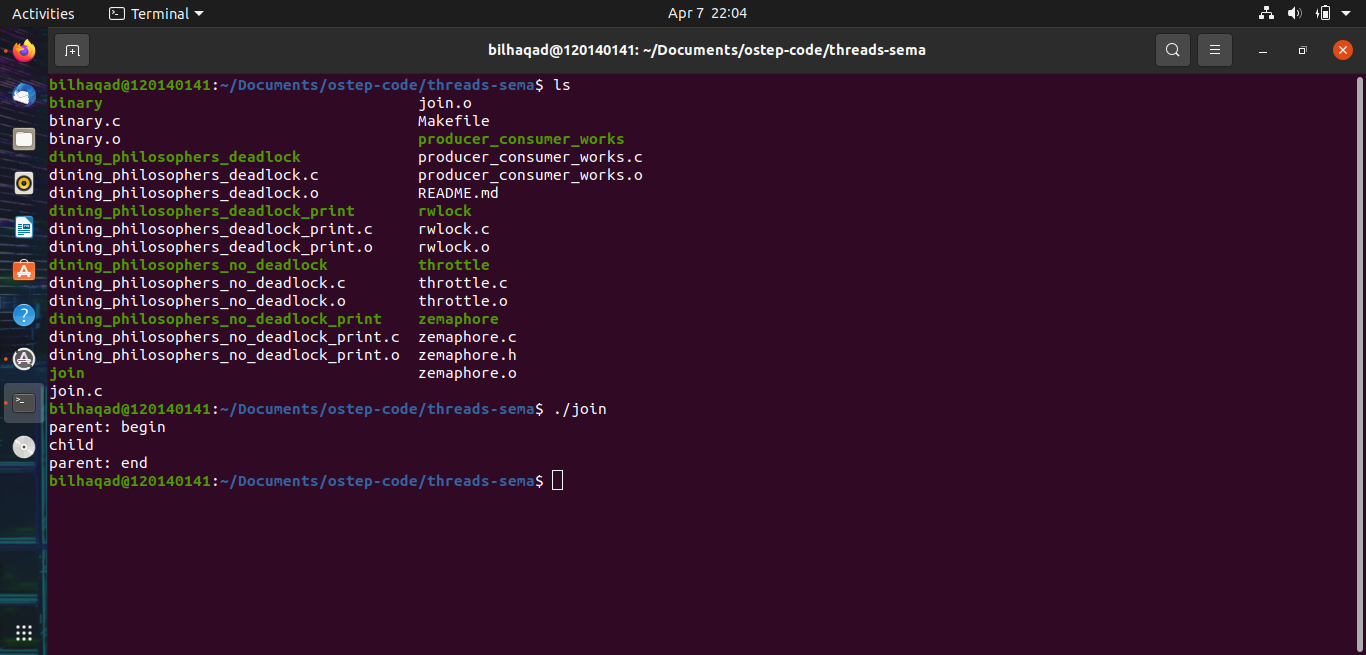
\includegraphics[width=0.8\textwidth]{Figure1/fork.png}
	\caption{\textit{Fork/Join}}
\end{figure}

\subsection{Penjelasan \textit{Fork/Join}} 
Semaphore merupakan sebuah struktur data komputer yang berguna dalam sinkronisasi proses dan berfungsi dalam memerintah program agar menjalankan proses.
Sebagai contohnya adalah saat suatu \textit{thread} sedang menunggu \textit{list} supaya \textit{list} tersebut berisi atau tidak keadaan kosong. Dari kondisi tersebut, 
semaphore tadi akan di definisikan dan di inisiasi menjadi 0 oleh \textit{Sem init}. Maksud dari proses tersebut ialah semaphore akan dibagi antara \textit{threads} pada proses
yang sama. Kemudian apabila pembuatan \textit{thread} sudah selesai akan dilanjutkan pemanggilan fungsi \textit{child} semaphore yang akan melakukan sinyal bahwa 
proses \textit{child} sudah selesai dan mulai me-\textit{return}. Apabila \textit{child} sudah selesai, maka semaphore akan melanjutkannya dan mengeluarkan \textit{output} 
"parent : end". \par
Pada implementasinya, terdapat fungsi \textit{Sem wait} dan \textit{Sem post} yang digunakan dalam menunggu kondisi \textit{child} dari \textit{parent} selesai eksekusi.
pada kode tersebut terlihat bahwa \textit{value} semaphore harus diubah menjadi 0 karena apabila kondisi tersebut tidak dilakukan akan membuat \textit{parent} memanggil fungsi 
\textit{Sem wait} duluan sebelum \textit{child} selesai memanggil fungsi \textit{Sem post}. Dan dari situ, dapat diketahui bila \textit{value} semaphore lebih dari 0 akan melakukan pengurangan 
untuk melakukan \textit{sleeps} selama 2 detik. Apabila \textit{value} semaphore sama dengan 0, maka program mulai menjalankan \textit{parent} dan selesai.


\section{Binary Semaphores}
\subsection{Source Code}
\begin{lstlisting}[language=C]
	#include <stdio.h>
	#include <stdlib.h>
	#include <pthread.h>
	#include <unistd.h>

	#include "common.h"
	#include "common_threads.h"

	#ifdef linux
	#include <semaphore.h>
	#elif __APPLE__
	#include "zemaphore.h"
	#endif

	sem_t mutex;
	volatile int counter = 0;

	void *child(void *arg) {
		int i;
		for (i = 0; i < 10000000; i++) {
		Sem_wait(&mutex);
		counter++;
		Sem_post(&mutex);
		}
		return NULL;
	}

	int main(int argc, char *argv[]) {
		Sem_init(&mutex, 1); 
		pthread_t c1, c2;
		Pthread_create(&c1, NULL, child, NULL);
		Pthread_create(&c2, NULL, child, NULL);
		Pthread_join(c1, NULL);
		Pthread_join(c2, NULL);
		printf("result: %d (should be 20000000)\n", counter);
		return 0;
	}
\end{lstlisting}

\subsection{Output}
\begin{figure}[h]
	\centering
	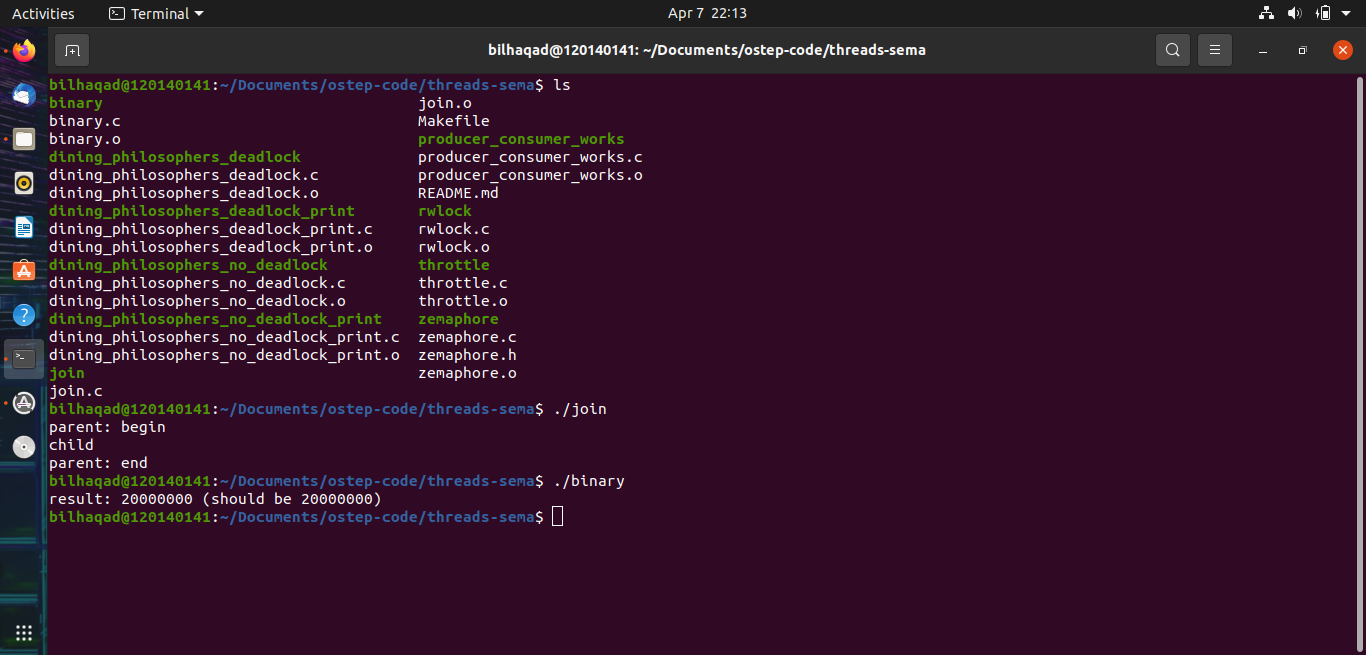
\includegraphics[width=0.8\textwidth]{Figure1/binary.png}
	\caption{\textit{Binary Semaphores}}
\end{figure}

\subsection{Penjelasan \textit{Binary Semaphores}}
Pada potongan kode di atas terdapat variabel \textit{Sem t mutex} atau bisa disebut dengan \textit{mutual exclusion} yang berfungsi dalam mengatur penggunaan \textit{resource}. \textit{mutex} tersebut ada agar mencegah sebuah
\textit{race condition}. Pada awalnya kita mendefinisikan dan menginisialisasikan semaphore \textit{mutex} tesebut dengan \textit{value} sebesar 1, kemudian dibuatlah \textit{thread} berinisial c1 dan c2 yang mana berguna dalam 
menjalankan fungsi \textit{child}. Selanjutntya, i akan di inisiasi pada perulangan sampai nilai i kurang dari 10000000 yang mana akan menjalankan \textit{Sem wait} dan di saat itu juga \textit{value} akan berkurang dan mulailah terjadi 
\textit{critical section}, akan ada penambahan nilai \textit{counter} yang kemudian semaphore memproses \textit{calling} dengan menambah \textit{value} dari semaphore tersebut sebagai tanda \textit{critical section} sudah selesai.
Berikutnya, program akan mengulangi proses tersebut hingga syarat telah tercapai yang kemudian akan dilanjutkan oleh \textit{thread} c2 melakukan fungsi \textit{child}. Bila sudah selesai, maka akan memulai \textit{return} ke fungsi \textit{main} 
yang akan menampilkan hasil dari \textit{counter} yang telah dijalankan dengan menampilkan \textit{output} senilai 20000000.

\section{Producer/Consumer}
\subsection{Source Code}
\begin{lstlisting}[language=C]
	#include <stdio.h>
	#include <unistd.h>
	#include <assert.h>
	#include <pthread.h>
	#include <stdlib.h>

	#include "common.h"
	#include "common_threads.h"

	#ifdef linux
	#include <semaphore.h>
	#elif __APPLE__
	#include "zemaphore.h"
	#endif

	int max;
	int loops;
	int *buffer;

	int use  = 0;
	int fill = 0;

	sem_t empty;
	sem_t full;
	sem_t mutex;

	#define CMAX (10)
	int consumers = 1;

	void do_fill(int value) {
		buffer[fill] = value;
		fill++;
		if (fill == max)
		fill = 0;
	}

	int do_get() {
		int tmp = buffer[use];
		use++;
		if (use == max)
		use = 0;
		return tmp;
	}

	void *producer(void *arg) {
		int i;
		for (i = 0; i < loops; i++) {
		Sem_wait(&empty);
		Sem_wait(&mutex);
		do_fill(i);
		Sem_post(&mutex);
		Sem_post(&full);
		}

		// end case
		for (i = 0; i < consumers; i++) {
		Sem_wait(&empty);
		Sem_wait(&mutex);
		do_fill(-1);
		Sem_post(&mutex);
		Sem_post(&full);
		}

		return NULL;
	}
																				
	void *consumer(void *arg) {
		int tmp = 0;
		while (tmp != -1) {
		Sem_wait(&full);
		Sem_wait(&mutex);
		tmp = do_get();
		Sem_post(&mutex);
		Sem_post(&empty);
		printf("%lld %d\n", (long long int) arg, tmp);
		}
		return NULL;
	}

	int main(int argc, char *argv[]) {
		if (argc != 4) {
		fprintf(stderr, "usage: %s <buffersize> <loops> <consumers>\n", argv[0]);
		exit(1);
		}
		max   = atoi(argv[1]);
		loops = atoi(argv[2]);
		consumers = atoi(argv[3]);
		assert(consumers <= CMAX);

		buffer = (int *) malloc(max * sizeof(int));
		assert(buffer != NULL);
		int i;
		for (i = 0; i < max; i++) {
		buffer[i] = 0;
		}

		Sem_init(&empty, max); // max are empty 
		Sem_init(&full, 0);    // 0 are full
		Sem_init(&mutex, 1);   // mutex

		pthread_t pid, cid[CMAX];
		Pthread_create(&pid, NULL, producer, NULL); 
		for (i = 0; i < consumers; i++) {
		Pthread_create(&cid[i], NULL, consumer, (void *) (long long int) i); 
		}
		Pthread_join(pid, NULL); 
		for (i = 0; i < consumers; i++) {
		Pthread_join(cid[i], NULL); 
		}
		return 0;
	}
\end{lstlisting}
\subsection{Output}
\begin{figure}[h]
	\centering
	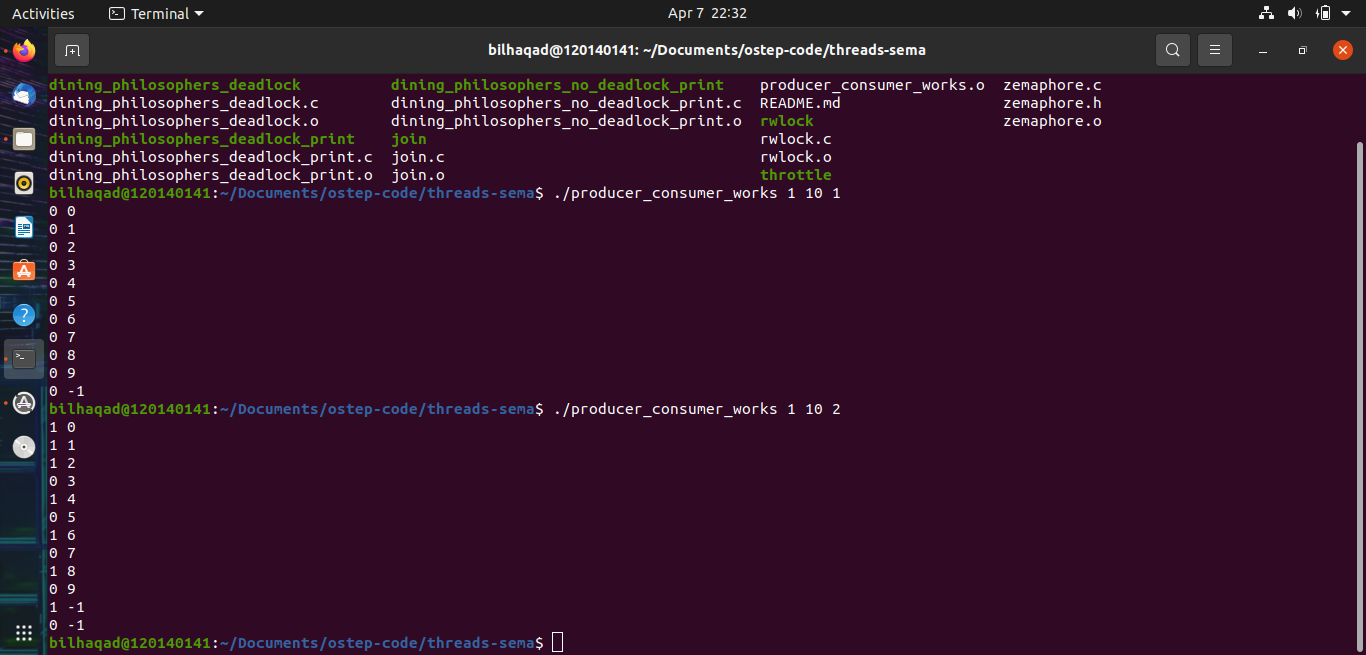
\includegraphics[width=0.8\textwidth]{Figure1/produce.png}
	\caption{\textit{Producer/Consumer}}
\end{figure}

\subsection{Penjelasan \textit{Producer/Consumer}}
Pada program implementasi \textit{Producer/Consumer} ini bisa kita sebut dengan \textit{bounded buffer}. Isi program tersebut ialah memanggil, mengurangi, mengahalngi konsumer, dan menunggu \textit{thread} lain agar dapat memanggil \textit{Sem post} saat terjadi \textit{full}. 
Selanjutntya, program akan memulai fungsi \textit{procedure} yang berguna dalam memanggil \textit{Sem wait(empty)} dan \textit{Sem post(mutex)}. Pada fungsi \textit{procedur} juga menjalankan terus sampai \textit{empty} tadi menjadi \textit{max}. \textit{Producer} akan melakukan pengisian 
dengan fungsi \textit{do fill} di \textit{entry} pertama \textit{buffer} setelah \textit{empty} berkurang hingga mencapai nilai 0. Berikutnya, \textit{producer} akan terus berjalan sampai suatu saat nanti memanggil \textit{Sem post(mutex)} dan \textit{Sem post(full)} yang mana akan mengganti 
nilai \textit{value full} dari nilai -1 menjadi 0. Sehingga, \textit{Consumer} akan melakukan fungsi \textit{looping} ulang dan memblok dengan \textit{value empty} semaphore bernilai kosong. \par
Apabila terjadi kondisi saat \textit{producer interrupted}, maka fungsi \textit{Consumer} mulai berjalan dengan kembalinya dari saat \textit{Sem wait(full)}, lalu akan memakai \textit{buffer} oleh berjalannya fungsi \textit{do get}. Kondisi dua \textit{producer} akan \textit{interrupted} apabila keduanya 
menjalankan fungsi \textit{do fill} pada waktu yang sama. Kondisi \textit{interruped} juga terjadi jika \textit{producer} yang ke-1 mengisi \textit{entry buffer} pertama kali, saat belum selesai dalam kesempatan mengisinya, maka \textit{producer} ke-1 akan ter-\textit{interruped}. Pada saat itulah \textit{producer} 
ke-2 menjalankan fungsi \textit{do fill} yang mana memasukkan elemen ke \textit{buffer}, kondisi tersebut berarti bahwa data lama akan terganti dengan yang baru. Oleh sebab itu, dibutuhkannya \textit{binary semaphore} dan ditambahnya \textit{locks} agar menghindarinya \textit{deadlock}. Dari situ, \textit{consumer} 
menjalankan yang pertama dengan memanggil \textit{Sem wait(full)} akbiat belum terdapatnya data. Dengan adanya pemanggilan tersebut, \textit{consumer} akan melakukan blok, selanjutnya \textit{producer} berjalan yang mana akan memulai \textit{consumer thread} dan memanggil \textit{Sem wait(mutex)} dengan \textit{producer} 
yang mengalami buntu atau \textit{stuck}. Pada program di atas terdapat juga \textit{cycle} yang simpel, \textit{consumer} menahan mutex agar menunggu untuk diberikan sinyal \textit{full}. Faktanya \textit{producer} bisa saja memanggil sinyal \textit{full}, tetapi tetap menunggu hingga \textit{consumer} dan \textit{producer} mengalami \textit{deadlock}. Oleh karena itu, 
dibutuhkannya pengurangan \textit{lock} dengan memindahkan \textit{mutex} dan melepaskannya pada sekitar \textit{critical section} akan menghasilkan \textit{working bounded buffer}.

\newpage
\section{Reader/Writer Locks}
\subsection{Source Code}
\begin{lstlisting}[language=C]
	#include <stdio.h>
	#include <stdlib.h>
	#include <pthread.h>
	#include <unistd.h>
	
	#include "common.h"
	#include "common_threads.h"
	
	#ifdef linux
	#include <semaphore.h>
	#elif __APPLE__
	#include "zemaphore.h"
	#endif
	
	typedef struct _rwlock_t {
		sem_t writelock;
		sem_t lock;
		int readers;
	} rwlock_t;
	
	void rwlock_init(rwlock_t *lock) {
		lock->readers = 0;
		Sem_init(&lock->lock, 1); 
		Sem_init(&lock->writelock, 1); 
	}
	
	void rwlock_acquire_readlock(rwlock_t *lock) {
		Sem_wait(&lock->lock);
		lock->readers++;
		if (lock->readers == 1)
		Sem_wait(&lock->writelock);
		Sem_post(&lock->lock);
	}
	
	void rwlock_release_readlock(rwlock_t *lock) {
		Sem_wait(&lock->lock);
		lock->readers--;
		if (lock->readers == 0)
		Sem_post(&lock->writelock);
		Sem_post(&lock->lock);
	}
	
	void rwlock_acquire_writelock(rwlock_t *lock) {
		Sem_wait(&lock->writelock);
	}
	
	void rwlock_release_writelock(rwlock_t *lock) {
		Sem_post(&lock->writelock);
	}
	
	int read_loops;
	int write_loops;
	int counter = 0;
	
	rwlock_t mutex;
	
	void *reader(void *arg) {
		int i;
		int local = 0;
		for (i = 0; i < read_loops; i++) {
		rwlock_acquire_readlock(&mutex);
		local = counter;
		rwlock_release_readlock(&mutex);
		printf("read %d\n", local);
		}
		printf("read done: %d\n", local);
		return NULL;
	}
	
	void *writer(void *arg) {
		int i;
		for (i = 0; i < write_loops; i++) {
		rwlock_acquire_writelock(&mutex);
		counter++;
		rwlock_release_writelock(&mutex);
		}
		printf("write done\n");
		return NULL;
	}
	
	int main(int argc, char *argv[]) {
		if (argc != 3) {
		fprintf(stderr, "usage: rwlock readloops writeloops\n");
		exit(1);
		}
		read_loops = atoi(argv[1]);
		write_loops = atoi(argv[2]);
		
		rwlock_init(&mutex); 
		pthread_t c1, c2;
		Pthread_create(&c1, NULL, reader, NULL);
		Pthread_create(&c2, NULL, writer, NULL);
		Pthread_join(c1, NULL);
		Pthread_join(c2, NULL);
		printf("all done\n");
		return 0;
	}
\end{lstlisting}

\subsection{Output}
\begin{figure}[h]
	\centering
	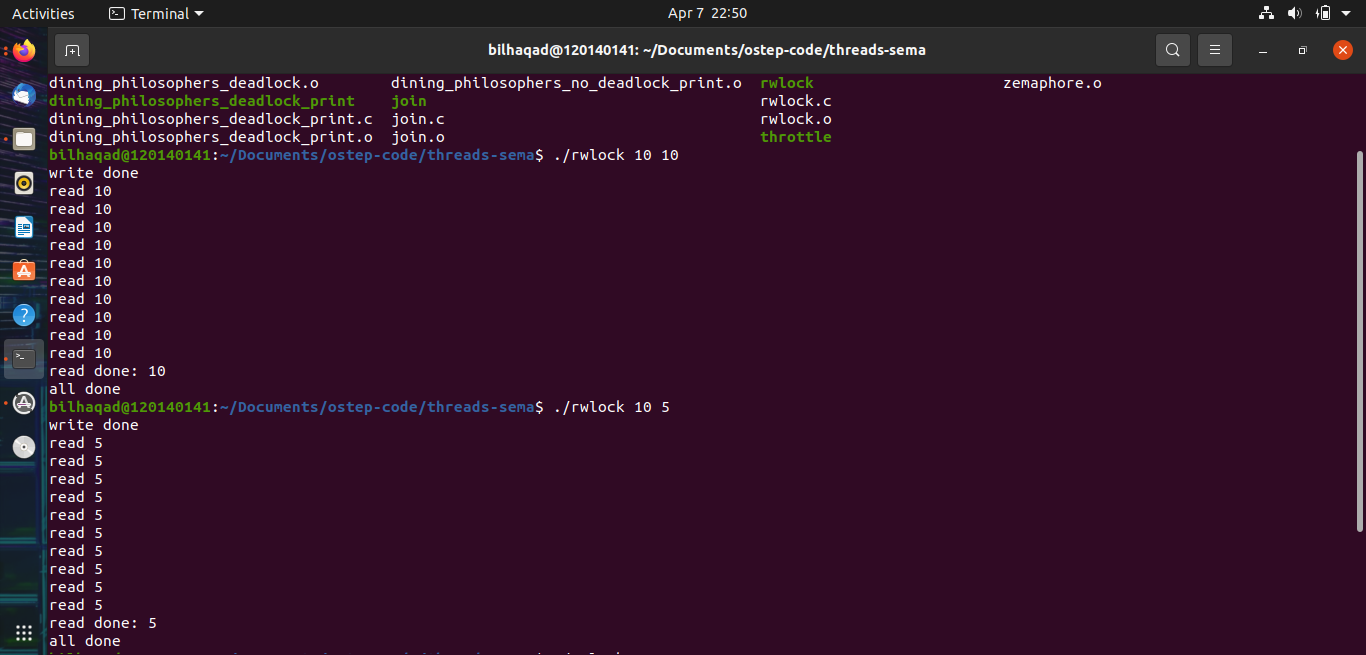
\includegraphics[width=0.75\textwidth]{Figure1/rwlock.png}
	\caption{\textit{Reader/Writer Locks}}
\end{figure}

\newpage
\subsection{Penjelasan \textit{Reader/Writer Locks}}
Pada program implementasi \textit{Reader/Writer Locks}, dapat dilihat bahwa terdapat \textit{classic problem} dari \textit{flexible locking primitive} yang menunjukkan bahwa 
akses struktur data berbeda perlu dibutuhkannya kunci spesial yang dibuat sebagai pembantu tipe operasi seperti \textit{reader/writer locks}. Apabila suatu saat \textit{thread} 
memperbaruit struktur datanya agar dapat memanggil pasangan operasi sinkronisasi \textit{rwlock acquire writelock} yang mana berfungsi dalam mendapatkan \textit{write lock} dan 
\textit{rwlock release writelock} untuk melepaskannya. Secara umumnya, semaphore \textit{writelock} untuk memastikan hanya satu \textit{writer} saja yang mendapatkan \textit{lock} dan 
memperbarui struktur datanya dengan masuknya ke \textit{critical section}. \par
Kondisi ketika \textit{lock} didapatkan, \textit{reader} yang pertama akan mendapatkan \textit{lock} tersebut dan mulai menambahkan variabel pembaca agar dapat melacak berapa pembaca yang 
ada saat ini pada struktur data. Perlu diperhatikan bahwa \textit{rwlock acquire readlock} terjadi saat pembaca ke-1 mendapatkan \textit{lock} dan \textit{writelock} dengan memanggil \text{Sem wait} 
pada saat semaphore \textit{writelock} yang akan dilepaskan \textit{lock}-nya saat memanggil \textit{Sem post}. \par
Selanjutnya, saat semua \textit{threads} diharapkan mendapatakan \textit{writelock} wajib menunggu sampai semua \textit{reader} telahh selesai dijalankan. Saat urutan terakhir keluar dari \textit{critical section}, akan 
memanggil \textit{Sem post} pada \textit{writelock} dan mulai mengaktifkannya \textit{writer} dengan menunggu dapatnya \textit{lock}. Pada akhirnya, pencatatan \textit{readwriter locks} wajib dilakukan secara hati-hati karena 
hal tersebut akan menambahkan \textit{overhead} dan tidak menambah performa yang berguna sebagai komparansi di \textit{simple} dan \textit{fast locking primptive}.


\section{Dining Philosophers}
\subsection{Deadlock}
\subsubsection{Source Code}
\begin{lstlisting}{language=C}
	#include <stdio.h>
	#include <stdlib.h>
	#include <pthread.h>
	
	#include "common.h"
	#include "common_threads.h"
	
	#ifdef linux
	#include <semaphore.h>
	#elif __APPLE__
	#include "zemaphore.h"
	#endif
	
	typedef struct {
		int num_loops;
		int thread_id;
	} arg_t;
	
	sem_t forks[5];
	sem_t print_lock;
	
	void space(int s) {
		Sem_wait(&print_lock);
		int i;
		for (i = 0; i < s * 10; i++)
		printf(" ");
	}
	
	void space_end() {
		Sem_post(&print_lock);
	}
	
	int left(int p)  {
		return p;
	}
	
	int right(int p) {
		return (p + 1) % 5;
	}
	
	void get_forks(int p) {
		space(p); printf("%d: try %d\n", p, left(p)); space_end();
		Sem_wait(&forks[left(p)]);
		space(p); printf("%d: try %d\n", p, right(p)); space_end();
		Sem_wait(&forks[right(p)]);
	}
	
	void put_forks(int p) {
		Sem_post(&forks[left(p)]);
		Sem_post(&forks[right(p)]);
	}
	
	void think() {
		return;
	}
	
	void eat() {
		return;
	}
	
	void *philosopher(void *arg) {
		arg_t *args = (arg_t *) arg;
	
		space(args->thread_id); printf("%d: start\n", args->thread_id); space_end();
	
		int i;
		for (i = 0; i < args->num_loops; i++) {
		space(args->thread_id); printf("%d: think\n", args->thread_id); space_end();
		think();
		get_forks(args->thread_id);
		space(args->thread_id); printf("%d: eat\n", args->thread_id); space_end();
		eat();
		put_forks(args->thread_id);
		space(args->thread_id); printf("%d: done\n", args->thread_id); space_end();
		}
		return NULL;
	}
																				 
	int main(int argc, char *argv[]) {
		if (argc != 2) {
		fprintf(stderr, "usage: dining_philosophers <num_loops>\n");
		exit(1);
		}
		printf("dining: started\n");
		
		int i;
		for (i = 0; i < 5; i++) 
		Sem_init(&forks[i], 1);
		Sem_init(&print_lock, 1);
	
		pthread_t p[5];
		arg_t a[5];
		for (i = 0; i < 5; i++) {
		a[i].num_loops = atoi(argv[1]);
		a[i].thread_id = i;
		Pthread_create(&p[i], NULL, philosopher, &a[i]);
		}
	
		for (i = 0; i < 5; i++) 
		Pthread_join(p[i], NULL); 
	
		printf("dining: finished\n");
		return 0;
	}
\end{lstlisting}

\subsubsection{Output}
\begin{figure}[h]
	\centering
	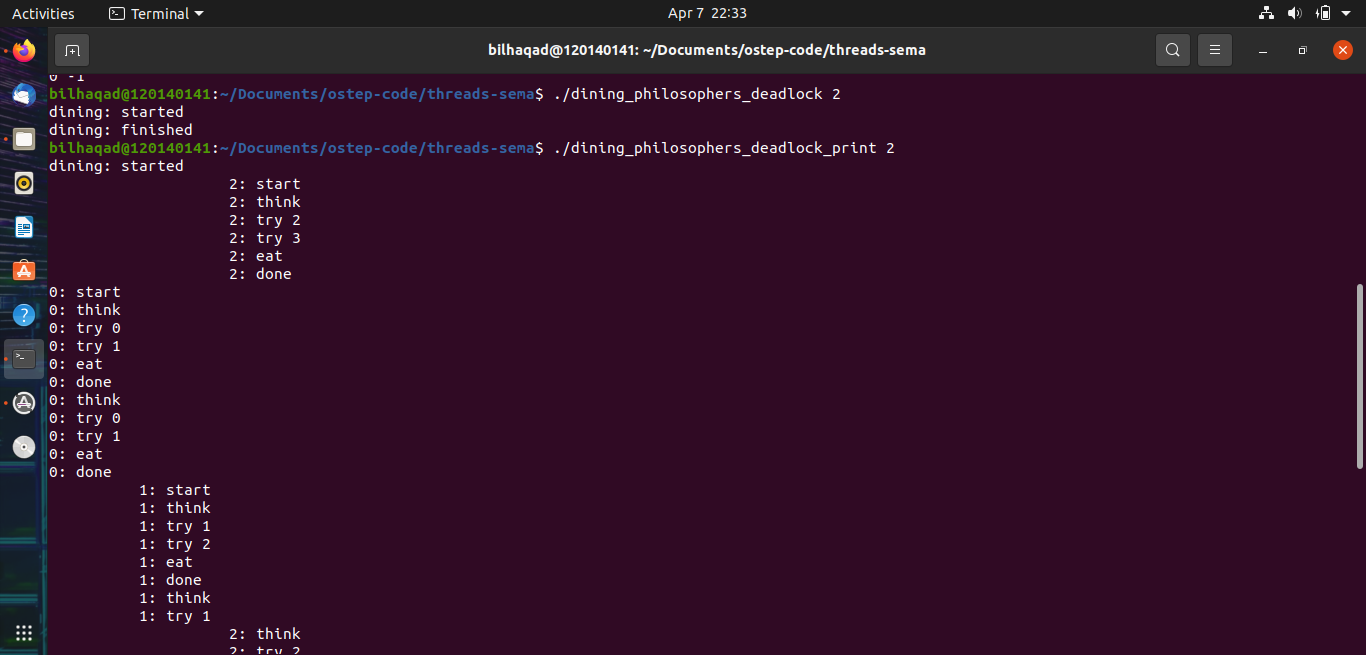
\includegraphics[width=0.8\textwidth]{Figure1/dining_deadlock1.png}
	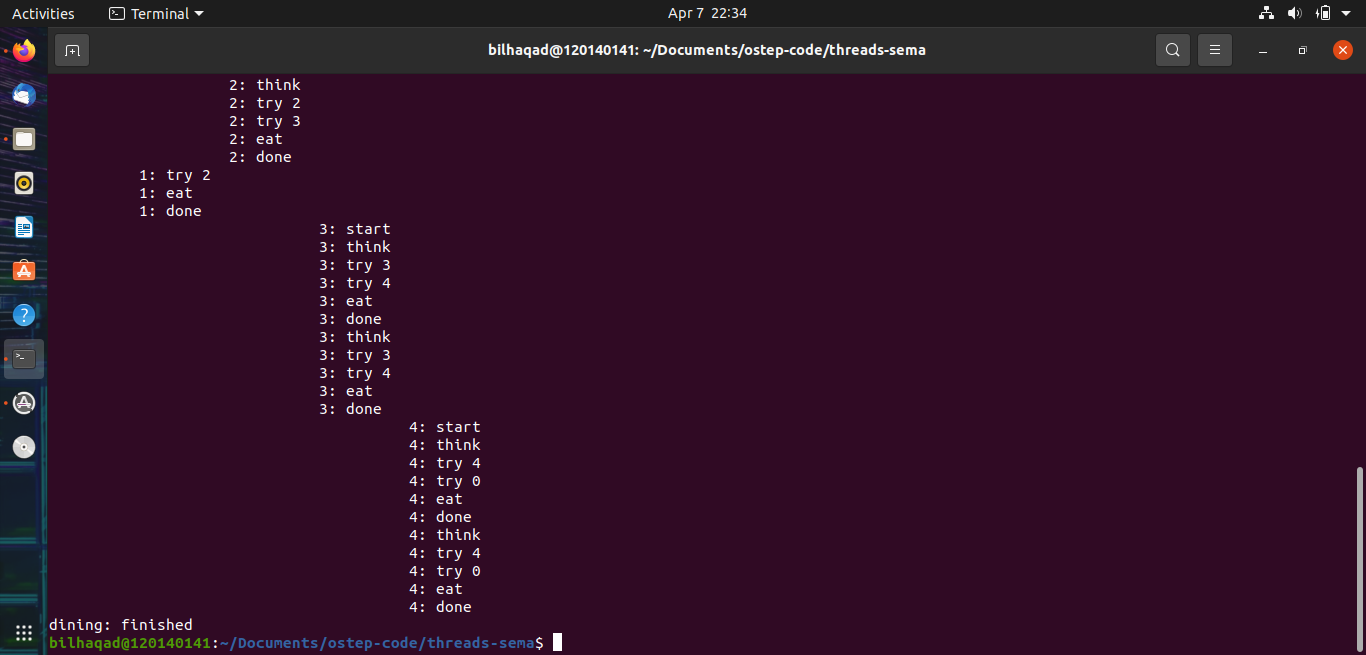
\includegraphics[width=0.8\textwidth]{Figure1/dining_deadlock2.png}
\end{figure}

\subsubsection{Penjelasan \textit{Dining Philosophers Deadlock}}
Pada implementasi program \textit{Dining Philosopher Deadlock} mempunyai cerita yang menarik dibelakangnya. Terdapat suatu masalah konkurensi yang dulu terkenal yang hanya diselesaikan 
oleh djikstra, masalah tersebut terkenal karena seru dan menarik secara intelektual yaitu dengan nama \textit{Philosopher problem}. Kondisinya ketika 5 \textit{philoshoper} yang duduk mengelilingi 
meja bundar terdapat sepasang \textit{philosopher single fork} yang mana untuk memulai makan dibutuhkan sepasang \textit{forks} satu di sebelah kanan dan satu di sebelah kiri. Dengan adanya solusi oleh 
Downey, diperlukannya beberapa fungsi bantu yang disebut \textit{left} dam \textit{right}. \par
Kondisi ketika \textit{philosopher P} diminta agar merujuk ke \textit{fork} kiri akan memulai memanggil fungsi \textit{left}, dan sebaliknya jika diminta merujuk ke \textit{fork} kanan akan memanggil fungsi 
\textit{right}. Terdapat \textit{modulo} yang mana menangani satu persoalan yaitu \textit{philosopher} akhir dengan P sama dengan 4 mengambil \textit{fork} bagian kanan saat \textit{fork} bernilai kosong.

\subsection{No Deadlock}
\subsubsection{Source Code}
\begin{lstlisting}[language=C]
	#include <stdio.h>
	#include <stdlib.h>
	#include <pthread.h>

	#include "common.h"
	#include "common_threads.h"

	#ifdef linux
	#include <semaphore.h>
	#elif __APPLE__
	#include "zemaphore.h"
	#endif

	typedef struct {
		int num_loops;
		int thread_id;
	} arg_t;

	sem_t forks[5];
	sem_t print_lock;

	void space(int s) {
		Sem_wait(&print_lock);
		int i;
		for (i = 0; i < s * 10; i++)
		printf(" ");
	}

	void space_end() {
		Sem_post(&print_lock);
	}

	int left(int p)  {
		return p;
	}

	int right(int p) {
		return (p + 1) % 5;
	}

	void get_forks(int p) {
		if (p == 4) {
		space(p); printf("4 try %d\n", right(p)); space_end();
		Sem_wait(&forks[right(p)]);
		space(p); printf("4 try %d\n", left(p)); space_end();
		Sem_wait(&forks[left(p)]);
		} else {
		space(p); printf("try %d\n", left(p)); space_end();
		Sem_wait(&forks[left(p)]);
		space(p); printf("try %d\n", right(p)); space_end();
		Sem_wait(&forks[right(p)]);
		}
	}

	void put_forks(int p) {
		Sem_post(&forks[left(p)]);
		Sem_post(&forks[right(p)]);
	}

	void think() {
		return;
	}

	void eat() {
		return;
	}

	void *philosopher(void *arg) {
		arg_t *args = (arg_t *) arg;

		space(args->thread_id); printf("%d: start\n", args->thread_id); space_end();

		int i;
		for (i = 0; i < args->num_loops; i++) {
		space(args->thread_id); printf("%d: think\n", args->thread_id); space_end();
		think();
		get_forks(args->thread_id);
		space(args->thread_id); printf("%d: eat\n", args->thread_id); space_end();
		eat();
		put_forks(args->thread_id);
		space(args->thread_id); printf("%d: done\n", args->thread_id); space_end();
		}
		return NULL;
	}
																				
	int main(int argc, char *argv[]) {
		if (argc != 2) {
		fprintf(stderr, "usage: dining_philosophers <num_loops>\n");
		exit(1);
		}
		printf("dining: started\n");
		
		int i;
		for (i = 0; i < 5; i++) 
		Sem_init(&forks[i], 1);
		Sem_init(&print_lock, 1);

		pthread_t p[5];
		arg_t a[5];
		for (i = 0; i < 5; i++) {
		a[i].num_loops = atoi(argv[1]);
		a[i].thread_id = i;
		Pthread_create(&p[i], NULL, philosopher, &a[i]);
		}

		for (i = 0; i < 5; i++) 
		Pthread_join(p[i], NULL); 

		printf("dining: finished\n");
		return 0;
	}
\end{lstlisting}

\newpage
\subsubsection{Output}
\begin{figure}[h]
	\centering
	\begin{subfigure}[b]{0.4\textwidth}
		\centering
		\def\svgwidth{\columnwidth}
		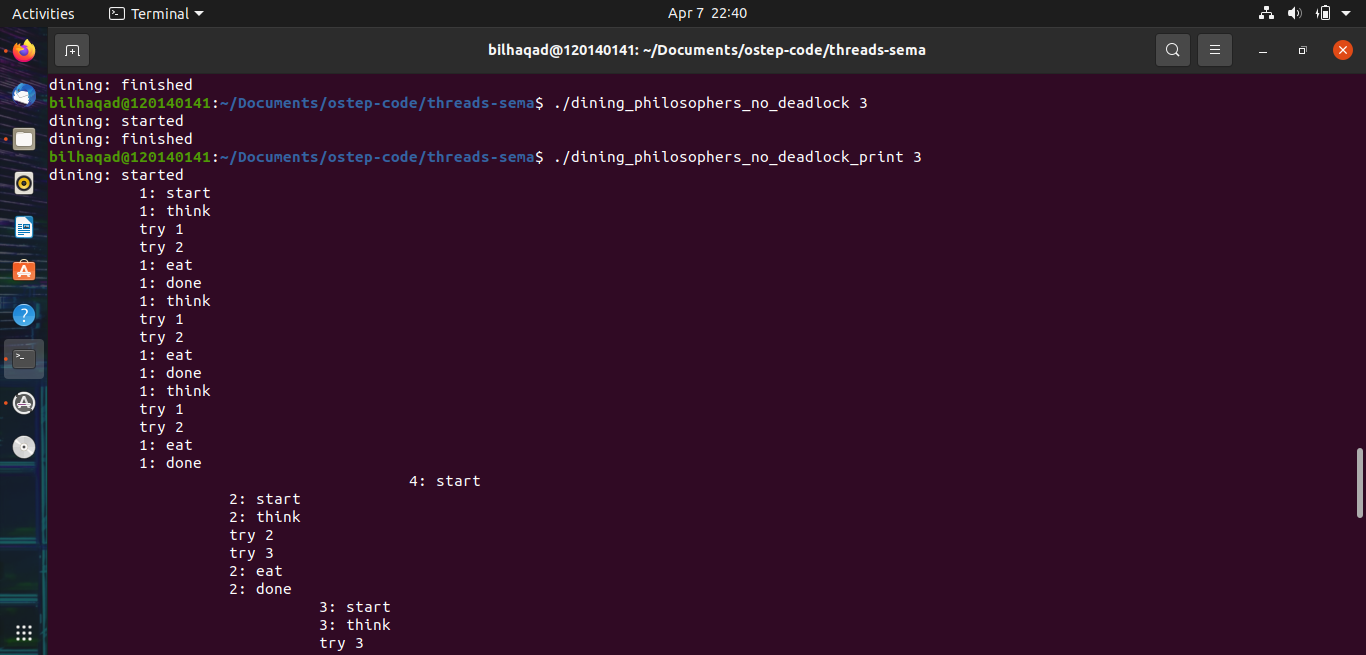
\includegraphics[width=1\textwidth]{Figure1/dining_nodeadlock1.png}
		\label{fig:nodeadlock1}
	\end{subfigure}
	\qquad %add desired spacing between images, e. g. ~, \quad, \qquad, \hfill etc. 
	%(or a blank line to force the subfigure onto a new line)
	\begin{subfigure}[b]{0.4\textwidth}
		\centering
		\def\svgwidth{\columnwidth}
		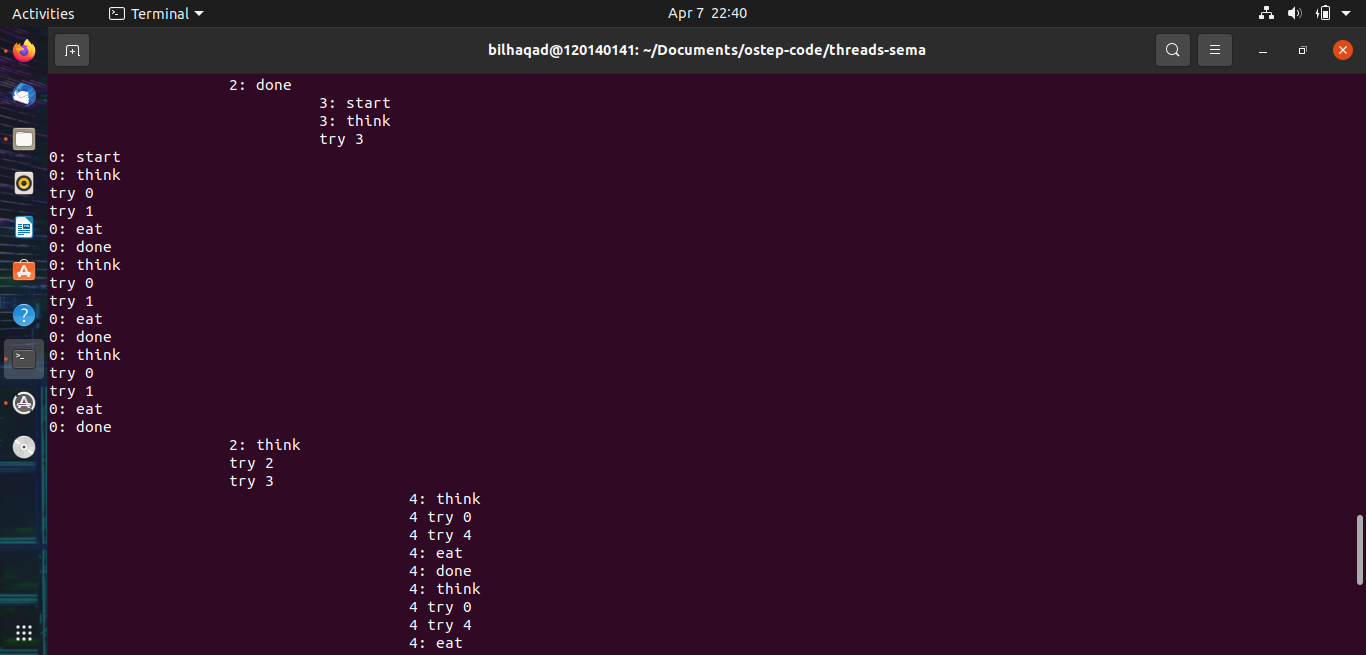
\includegraphics[width=1\textwidth]{Figure1/dining_nodeadlock2.png}
		\label{fig:nodeadlock2}
	\end{subfigure}
	\begin{subfigure}[b]{0.4\textwidth}
		\centering
		\def\svgwidth{\columnwidth}
		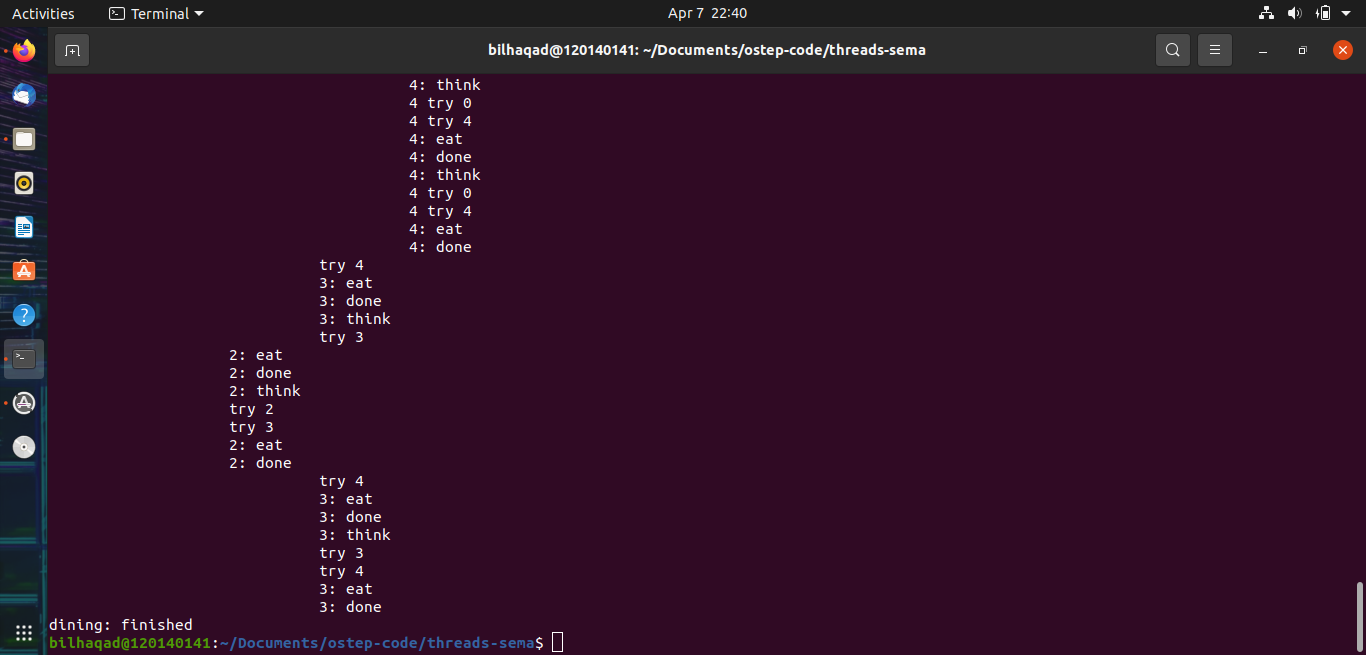
\includegraphics[width=1\textwidth]{Figure1/dining_nodeadlock3.png}
		\label{fig:nodeadlock3}
	\end{subfigure}
	\caption{Dining Philosophers No Deadlock}\label{fig:aug}
\end{figure}

\subsubsection{Penjelasan \textit{Dining Philosophers No Deadlock}}
Pada implementasi program \textit{Dining Philosophers No Deadlock} di atas menjelaskan tentang percobaan menginisialisasi setiap semaphore di \textit{fork array} agar bernilai 1.
Perlu kita ketahui bahwa \textit{philosopher} mempunyai angka dan juga kita bisa menuliskan \textit{get forks} dan \textit{put forks} secara terus-menerus. Kemudian, kita memerlukan 
\textit{lock} untuk mendapati \textit{forks} dengan mendapatkan \textit{forks} sebelah kiri dan dilanjutkan sebelah kanan. Kemudian pastinya ketika kita selesai memakainya pasti akan kita 
lepaskan, tetapi kondisi tersebut tidak terjadi karena adanya \textit{deadlock}. Apabila setiap \textit{philosopher} mengambil \textit{fork} sebelah kiri terlebih dahulu sebelum bisa mengambil 
\textit{fork} sebelah kanan, maka menyebabkan \textit{stuck} dan dapat menahan satu \textit{fork} yang mana membuat \textit{fork} lainnya menunggu untuk selamanya. \par
Contoh dari penggambarannya ialah misalkan \textit{philosopher} 0 mengambil \textit{fork} 0, \textit{philosopher} 1 mengambil \textit{fork} 1, \textit{philosopher} 2 mengambil \textit{fork} 2, dan 
\textit{philoshoper} 3 mengambil \textit{fork} 3 akan menyebabkan semua \textit{philosopher} terperangkap atau \textit{stuck} karena tidak ada ruangan pada \textit{philosopher}. \par
Dari permasalahan tersebut Djikstra menemukan solusinya dengan mengganti \textit{fork} mendapatkan satu \textit{philosopher} saja. Dengan asumsi 4 \textit{philosopher} mengambil \textit{fork} melalui 
aturan yang berbeda dengan sebelumnya, hal tersebut disebabkan karena \textit{philoshoper} akhir mengambil sebelah kanan terlebih dahulu seelum sebelah kiri. Pasalnya, tidak ada aturan \textit{philosopher} 
mengambil satu \textit{fork} dan mengalami \textit{stuck} dengan menunggu \textit{fork} lainnya. Oleh karena itu, adanya siklus \textit{waiting} ini merusak prosesnya.

\newpage
\section{Kesimpulan}
	Pada Hands On 2 ini, yang saya dapatkan setelah mengerjakannya ialah saya dapat mengerti lebih dalam dengan materi 
	\textit{Synchronisation and Deadlock} dengan adanya pemberian kode program dari suatu \textit{programmer} yang membuat 
	programnya sesuai dengan impelementasi materi tersebut. Dan begitu juga saya mengerti tentang adanya penggunaan Semaphore 
	pada program yang telah dijalankan. Dengan demikian, saya dapat menejelajahi lebih dalam terkait dengan materi sinkronisasi 
	dan \textit{deadlock} ini atas tugas Hands On 2 yant telah diberikan.
		
\section{Link GitHub}
	Link GitHub dari Hands On 2 ini : \href{https://github.com/BilhaqAD07/Sistem-Operasi.git}{Klik disini}


\newpage
\bibliographystyle{IEEEtran}
\bibliography{Referensi}
\end{document}